\quiz{2022-119}{https://net-sci-questions.blogspot.com/2022/05/2022-099.htmll}

Starting from the node indicated as `start', use DFS and label the nodes with their ending times. Which of the alternatives below corresponds to a possible answer?

\begin{figure}[H]
    \centering
    \includegraphics{images/119-0.png}
\end{figure}

Tip: the reverse order of finishing DFS times in a directed acyclic graph is a topological order.

\begin{enumerate}[label={\Alph*.}]

\raggedcolumns\begin{multicols}{2}
    \item \includegraphics[width=0.45\textwidth]{images/119-A.png}

    \item \includegraphics[width=0.45\textwidth]{images/119-B.png}
\end{multicols}

\raggedcolumns\begin{multicols}{2}
    \item \includegraphics[width=0.45\textwidth]{images/119-C.png}

    \item \includegraphics[width=0.45\textwidth]{images/119-D.png}
\end{multicols}

    \item None of the above
\end{enumerate}

Original ideia by: Filipe Maciel Roberto


\subsection*{Answer: C}

The given digraph is acyclic, therefore the finishing time must form a topological sorting of its vertices.

For \textbf{A.}, we have 18 as a successor to 19 in the topological order, but there's aa back arc from 18 to 19, invalidating this order.

For \textbf{B.}, there's an arc from 10 to 20. In fact, the start node must be the last with the largest finishing time.

For \textbf{C.}, the topological is valid:

\begin{figure}[H]
    \centering
    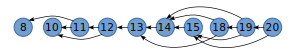
\includegraphics[width=0.95\textwidth]{images/119.pdf}
\end{figure}

For \textbf{D.}, the single invalid arc is from 8 to 12.
